\section{SOLID implementatie}
Tijdens het realiseren zijn de ontwerp principes van SOLID (zie \ref{subsecion:SoftwareArhitectuur} voor meer informatie) mee genomen.
In deze sectie wordt er meer ingezoomed naar de implementatie van de SOLID principes en hoe dat tot uiting is gekomen.

\whitespace
De software architectuur maakt gebruik van handlers.
Een hanlder is een encapsulatie van de buisness logica voor een bepaalde context.
Deze handler heeft maar één taak waardoor het aan het \textit{Single-responsibility principle} voldoet.
In het voorbeeld (figuur \ref{fig:ImplementationUpsertItemHandler}) is te zien dat deze handlers als taak heeft het upserten van Items.
In figuur \ref{fig:interfaceUpsertItemHandler} is te zien dat hij 2 methodes heeft, maar beide methodes hebben de zelfde \qw{taak} het upserten van items.

\whitespace
\begin{graphic}
    \captionsetup{type=figure}
    \caption{Visualisatie van fields}
    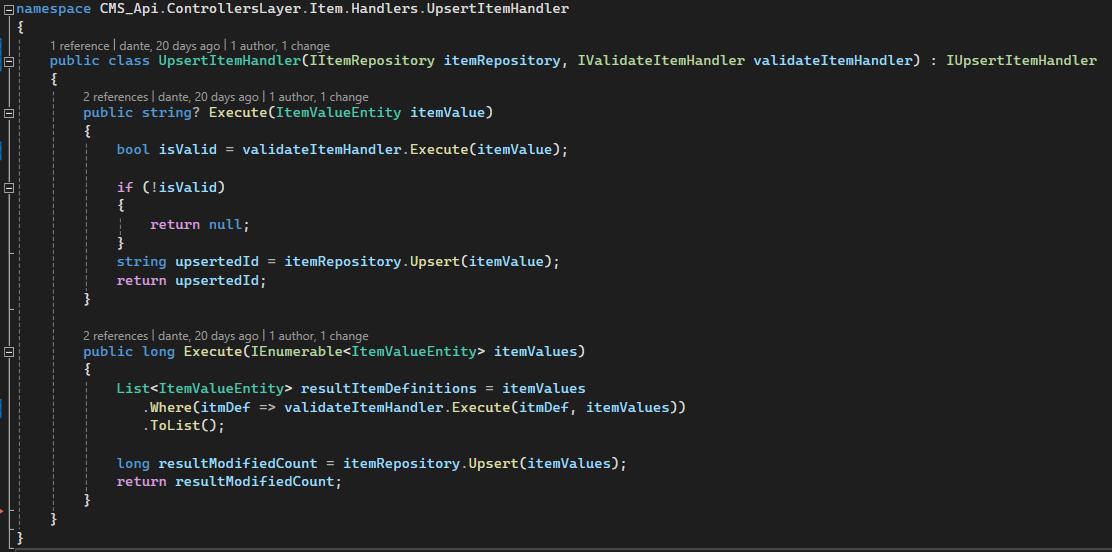
\includegraphics[scale=0.6]{ImplementationUpsertItemHandler.png}
    \label{fig:ImplementationUpsertItemHandler}
\end{graphic}

\whitespace[2]
\begin{graphic}
    \captionsetup{type=figure}
    \caption{Visualisatie van fields}
    \includegraphics[scale=0.6]{interfaceUpsertItemHandler.png}
    \label{fig:interfaceUpsertItemHandler}
\end{graphic}

\whitespace[2]
In de verschillende handlers wordt er gebruik gemaakt van het \textit{Open\slash Closed principle}.
Dit is gedaan zodat er makkelijk een nieuwe implementatie genjecteerd kan worden zonder de oude code base aan te passen.
De verschillende dependencies kunnen vervangen worden door een andere concrete implementaties.
Hierdoor wordt er ook voldaan aan het \textit{Liskov substitution principle}.
Omdat de handlers maar één taak hebben blijft hun interface erg klein (meestal 1 of 2 methoden).
Dit zorgt dat de interfaces erg gefoces blijven op hun taak en er dan voldaan wordt aan het \textit{Interface segrigation principle}
De injectie van de concrete implementatie wordt gedaan doormiddel van \textit{Dependency injection}.
Door gebruik te maken van \textit{depencency injection} wordt er ook voldaan aan het \textit{Depencency inversion principle}.

% \whitespace
\subsection{Repository pattern}
Om de datalaag en de logica van elkaar te scheiden is er gebruikt van een repository pattern \parencite{RepositoryPattern}.
Het repository pattern is een structureel design pattern dat de datalaag en logica van de applicatie scheidt.
Dit wordt bereikt door middel van een abstracte tussenlaag die communicatie mogelijk maakt tussen de logica en de datalaag.

\whitespace
Dit leidt tot een scheiding tussen de logica en de data, waardoor voldaan wordt aan het \textit{single responsibility principle}.
Dit resulteert in beter testbare code, wat de betrouwbaarheid van het programma verhoogt.
Bovendien voorkomt dit dat de codebase afhankelijk is van één specifieke databaseprovider.

\whitespace
Dit is geimplementeerd door de logica af te laten hangen van een interface inplaats van een concrete implementatie.
Vervolgens wordt bij initialisatie van de applicatie  een concrete versie \textit{gedependency inject}.
Een visualisatie van de geïmplementeerde versie is te zien in figuur \ref{fig:RepositoryPattern}

\whitespace[2]
\begin{graphic}
    \captionsetup{type=figure}
    \caption{Visualisatie van fields}
    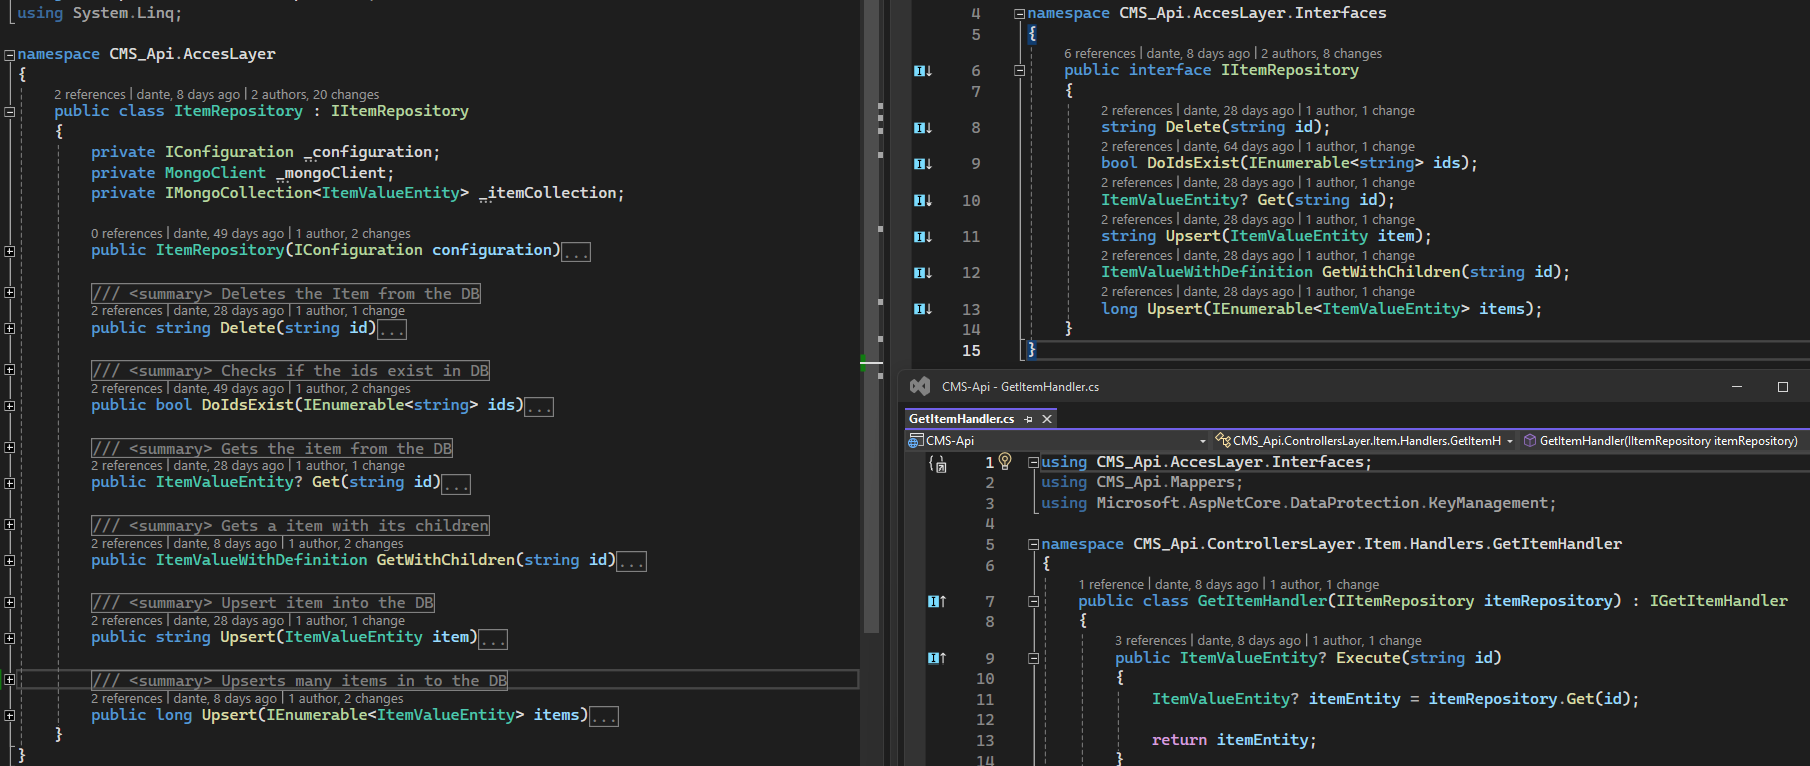
\includegraphics[scale=0.35]{ImplementationRepositoryPattern.png}
    \label{fig:RepositoryPattern}
\end{graphic}
